% Options for packages loaded elsewhere
\PassOptionsToPackage{unicode}{hyperref}
\PassOptionsToPackage{hyphens}{url}
\PassOptionsToPackage{dvipsnames,svgnames,x11names}{xcolor}
%
\documentclass[
  letterpaper,
  DIV=11,
  numbers=noendperiod]{scrreprt}

\usepackage{amsmath,amssymb}
\usepackage{iftex}
\ifPDFTeX
  \usepackage[T1]{fontenc}
  \usepackage[utf8]{inputenc}
  \usepackage{textcomp} % provide euro and other symbols
\else % if luatex or xetex
  \usepackage{unicode-math}
  \defaultfontfeatures{Scale=MatchLowercase}
  \defaultfontfeatures[\rmfamily]{Ligatures=TeX,Scale=1}
\fi
\usepackage{lmodern}
\ifPDFTeX\else  
    % xetex/luatex font selection
\fi
% Use upquote if available, for straight quotes in verbatim environments
\IfFileExists{upquote.sty}{\usepackage{upquote}}{}
\IfFileExists{microtype.sty}{% use microtype if available
  \usepackage[]{microtype}
  \UseMicrotypeSet[protrusion]{basicmath} % disable protrusion for tt fonts
}{}
\makeatletter
\@ifundefined{KOMAClassName}{% if non-KOMA class
  \IfFileExists{parskip.sty}{%
    \usepackage{parskip}
  }{% else
    \setlength{\parindent}{0pt}
    \setlength{\parskip}{6pt plus 2pt minus 1pt}}
}{% if KOMA class
  \KOMAoptions{parskip=half}}
\makeatother
\usepackage{xcolor}
\setlength{\emergencystretch}{3em} % prevent overfull lines
\setcounter{secnumdepth}{5}
% Make \paragraph and \subparagraph free-standing
\makeatletter
\ifx\paragraph\undefined\else
  \let\oldparagraph\paragraph
  \renewcommand{\paragraph}{
    \@ifstar
      \xxxParagraphStar
      \xxxParagraphNoStar
  }
  \newcommand{\xxxParagraphStar}[1]{\oldparagraph*{#1}\mbox{}}
  \newcommand{\xxxParagraphNoStar}[1]{\oldparagraph{#1}\mbox{}}
\fi
\ifx\subparagraph\undefined\else
  \let\oldsubparagraph\subparagraph
  \renewcommand{\subparagraph}{
    \@ifstar
      \xxxSubParagraphStar
      \xxxSubParagraphNoStar
  }
  \newcommand{\xxxSubParagraphStar}[1]{\oldsubparagraph*{#1}\mbox{}}
  \newcommand{\xxxSubParagraphNoStar}[1]{\oldsubparagraph{#1}\mbox{}}
\fi
\makeatother

\usepackage{color}
\usepackage{fancyvrb}
\newcommand{\VerbBar}{|}
\newcommand{\VERB}{\Verb[commandchars=\\\{\}]}
\DefineVerbatimEnvironment{Highlighting}{Verbatim}{commandchars=\\\{\}}
% Add ',fontsize=\small' for more characters per line
\usepackage{framed}
\definecolor{shadecolor}{RGB}{241,243,245}
\newenvironment{Shaded}{\begin{snugshade}}{\end{snugshade}}
\newcommand{\AlertTok}[1]{\textcolor[rgb]{0.68,0.00,0.00}{#1}}
\newcommand{\AnnotationTok}[1]{\textcolor[rgb]{0.37,0.37,0.37}{#1}}
\newcommand{\AttributeTok}[1]{\textcolor[rgb]{0.40,0.45,0.13}{#1}}
\newcommand{\BaseNTok}[1]{\textcolor[rgb]{0.68,0.00,0.00}{#1}}
\newcommand{\BuiltInTok}[1]{\textcolor[rgb]{0.00,0.23,0.31}{#1}}
\newcommand{\CharTok}[1]{\textcolor[rgb]{0.13,0.47,0.30}{#1}}
\newcommand{\CommentTok}[1]{\textcolor[rgb]{0.37,0.37,0.37}{#1}}
\newcommand{\CommentVarTok}[1]{\textcolor[rgb]{0.37,0.37,0.37}{\textit{#1}}}
\newcommand{\ConstantTok}[1]{\textcolor[rgb]{0.56,0.35,0.01}{#1}}
\newcommand{\ControlFlowTok}[1]{\textcolor[rgb]{0.00,0.23,0.31}{\textbf{#1}}}
\newcommand{\DataTypeTok}[1]{\textcolor[rgb]{0.68,0.00,0.00}{#1}}
\newcommand{\DecValTok}[1]{\textcolor[rgb]{0.68,0.00,0.00}{#1}}
\newcommand{\DocumentationTok}[1]{\textcolor[rgb]{0.37,0.37,0.37}{\textit{#1}}}
\newcommand{\ErrorTok}[1]{\textcolor[rgb]{0.68,0.00,0.00}{#1}}
\newcommand{\ExtensionTok}[1]{\textcolor[rgb]{0.00,0.23,0.31}{#1}}
\newcommand{\FloatTok}[1]{\textcolor[rgb]{0.68,0.00,0.00}{#1}}
\newcommand{\FunctionTok}[1]{\textcolor[rgb]{0.28,0.35,0.67}{#1}}
\newcommand{\ImportTok}[1]{\textcolor[rgb]{0.00,0.46,0.62}{#1}}
\newcommand{\InformationTok}[1]{\textcolor[rgb]{0.37,0.37,0.37}{#1}}
\newcommand{\KeywordTok}[1]{\textcolor[rgb]{0.00,0.23,0.31}{\textbf{#1}}}
\newcommand{\NormalTok}[1]{\textcolor[rgb]{0.00,0.23,0.31}{#1}}
\newcommand{\OperatorTok}[1]{\textcolor[rgb]{0.37,0.37,0.37}{#1}}
\newcommand{\OtherTok}[1]{\textcolor[rgb]{0.00,0.23,0.31}{#1}}
\newcommand{\PreprocessorTok}[1]{\textcolor[rgb]{0.68,0.00,0.00}{#1}}
\newcommand{\RegionMarkerTok}[1]{\textcolor[rgb]{0.00,0.23,0.31}{#1}}
\newcommand{\SpecialCharTok}[1]{\textcolor[rgb]{0.37,0.37,0.37}{#1}}
\newcommand{\SpecialStringTok}[1]{\textcolor[rgb]{0.13,0.47,0.30}{#1}}
\newcommand{\StringTok}[1]{\textcolor[rgb]{0.13,0.47,0.30}{#1}}
\newcommand{\VariableTok}[1]{\textcolor[rgb]{0.07,0.07,0.07}{#1}}
\newcommand{\VerbatimStringTok}[1]{\textcolor[rgb]{0.13,0.47,0.30}{#1}}
\newcommand{\WarningTok}[1]{\textcolor[rgb]{0.37,0.37,0.37}{\textit{#1}}}

\providecommand{\tightlist}{%
  \setlength{\itemsep}{0pt}\setlength{\parskip}{0pt}}\usepackage{longtable,booktabs,array}
\usepackage{calc} % for calculating minipage widths
% Correct order of tables after \paragraph or \subparagraph
\usepackage{etoolbox}
\makeatletter
\patchcmd\longtable{\par}{\if@noskipsec\mbox{}\fi\par}{}{}
\makeatother
% Allow footnotes in longtable head/foot
\IfFileExists{footnotehyper.sty}{\usepackage{footnotehyper}}{\usepackage{footnote}}
\makesavenoteenv{longtable}
\usepackage{graphicx}
\makeatletter
\newsavebox\pandoc@box
\newcommand*\pandocbounded[1]{% scales image to fit in text height/width
  \sbox\pandoc@box{#1}%
  \Gscale@div\@tempa{\textheight}{\dimexpr\ht\pandoc@box+\dp\pandoc@box\relax}%
  \Gscale@div\@tempb{\linewidth}{\wd\pandoc@box}%
  \ifdim\@tempb\p@<\@tempa\p@\let\@tempa\@tempb\fi% select the smaller of both
  \ifdim\@tempa\p@<\p@\scalebox{\@tempa}{\usebox\pandoc@box}%
  \else\usebox{\pandoc@box}%
  \fi%
}
% Set default figure placement to htbp
\def\fps@figure{htbp}
\makeatother
% definitions for citeproc citations
\NewDocumentCommand\citeproctext{}{}
\NewDocumentCommand\citeproc{mm}{%
  \begingroup\def\citeproctext{#2}\cite{#1}\endgroup}
\makeatletter
 % allow citations to break across lines
 \let\@cite@ofmt\@firstofone
 % avoid brackets around text for \cite:
 \def\@biblabel#1{}
 \def\@cite#1#2{{#1\if@tempswa , #2\fi}}
\makeatother
\newlength{\cslhangindent}
\setlength{\cslhangindent}{1.5em}
\newlength{\csllabelwidth}
\setlength{\csllabelwidth}{3em}
\newenvironment{CSLReferences}[2] % #1 hanging-indent, #2 entry-spacing
 {\begin{list}{}{%
  \setlength{\itemindent}{0pt}
  \setlength{\leftmargin}{0pt}
  \setlength{\parsep}{0pt}
  % turn on hanging indent if param 1 is 1
  \ifodd #1
   \setlength{\leftmargin}{\cslhangindent}
   \setlength{\itemindent}{-1\cslhangindent}
  \fi
  % set entry spacing
  \setlength{\itemsep}{#2\baselineskip}}}
 {\end{list}}
\usepackage{calc}
\newcommand{\CSLBlock}[1]{\hfill\break\parbox[t]{\linewidth}{\strut\ignorespaces#1\strut}}
\newcommand{\CSLLeftMargin}[1]{\parbox[t]{\csllabelwidth}{\strut#1\strut}}
\newcommand{\CSLRightInline}[1]{\parbox[t]{\linewidth - \csllabelwidth}{\strut#1\strut}}
\newcommand{\CSLIndent}[1]{\hspace{\cslhangindent}#1}

\KOMAoption{captions}{tableheading}
\makeatletter
\@ifpackageloaded{tcolorbox}{}{\usepackage[skins,breakable]{tcolorbox}}
\@ifpackageloaded{fontawesome5}{}{\usepackage{fontawesome5}}
\definecolor{quarto-callout-color}{HTML}{909090}
\definecolor{quarto-callout-note-color}{HTML}{0758E5}
\definecolor{quarto-callout-important-color}{HTML}{CC1914}
\definecolor{quarto-callout-warning-color}{HTML}{EB9113}
\definecolor{quarto-callout-tip-color}{HTML}{00A047}
\definecolor{quarto-callout-caution-color}{HTML}{FC5300}
\definecolor{quarto-callout-color-frame}{HTML}{acacac}
\definecolor{quarto-callout-note-color-frame}{HTML}{4582ec}
\definecolor{quarto-callout-important-color-frame}{HTML}{d9534f}
\definecolor{quarto-callout-warning-color-frame}{HTML}{f0ad4e}
\definecolor{quarto-callout-tip-color-frame}{HTML}{02b875}
\definecolor{quarto-callout-caution-color-frame}{HTML}{fd7e14}
\makeatother
\makeatletter
\@ifpackageloaded{bookmark}{}{\usepackage{bookmark}}
\makeatother
\makeatletter
\@ifpackageloaded{caption}{}{\usepackage{caption}}
\AtBeginDocument{%
\ifdefined\contentsname
  \renewcommand*\contentsname{Table of contents}
\else
  \newcommand\contentsname{Table of contents}
\fi
\ifdefined\listfigurename
  \renewcommand*\listfigurename{List of Figures}
\else
  \newcommand\listfigurename{List of Figures}
\fi
\ifdefined\listtablename
  \renewcommand*\listtablename{List of Tables}
\else
  \newcommand\listtablename{List of Tables}
\fi
\ifdefined\figurename
  \renewcommand*\figurename{Figure}
\else
  \newcommand\figurename{Figure}
\fi
\ifdefined\tablename
  \renewcommand*\tablename{Table}
\else
  \newcommand\tablename{Table}
\fi
}
\@ifpackageloaded{float}{}{\usepackage{float}}
\floatstyle{ruled}
\@ifundefined{c@chapter}{\newfloat{codelisting}{h}{lop}}{\newfloat{codelisting}{h}{lop}[chapter]}
\floatname{codelisting}{Listing}
\newcommand*\listoflistings{\listof{codelisting}{List of Listings}}
\makeatother
\makeatletter
\makeatother
\makeatletter
\@ifpackageloaded{caption}{}{\usepackage{caption}}
\@ifpackageloaded{subcaption}{}{\usepackage{subcaption}}
\makeatother

\usepackage{bookmark}

\IfFileExists{xurl.sty}{\usepackage{xurl}}{} % add URL line breaks if available
\urlstyle{same} % disable monospaced font for URLs
\hypersetup{
  pdftitle={Philosophy of Science},
  pdfauthor={Thought and Reason},
  colorlinks=true,
  linkcolor={blue},
  filecolor={Maroon},
  citecolor={Blue},
  urlcolor={Blue},
  pdfcreator={LaTeX via pandoc}}


\title{Philosophy of Science}
\author{Thought and Reason}
\date{2025-04-07}

\begin{document}
\maketitle

\renewcommand*\contentsname{Table of contents}
{
\hypersetup{linkcolor=}
\setcounter{tocdepth}{2}
\tableofcontents
}

\bookmarksetup{startatroot}

\chapter*{Preface (Önsöz)}\label{preface-uxf6nsuxf6z}
\addcontentsline{toc}{chapter}{Preface (Önsöz)}

\markboth{Preface (Önsöz)}{Preface (Önsöz)}

\bookmarksetup{startatroot}

\chapter*{Content}\label{content}
\addcontentsline{toc}{chapter}{Content}

\markboth{Content}{Content}

This site will feature discussions on

\begin{itemize}
\tightlist
\item
  Philosophy of science
\item
  The use of language (formal, and natural) in sciences
\item
  Mathematics
\item
  The use of mathematics in sciences
\item
  The Islamic philosophy
\end{itemize}

\bookmarksetup{startatroot}

\chapter*{Contact}\label{contact}
\addcontentsline{toc}{chapter}{Contact}

\markboth{Contact}{Contact}

To send your comments or to contribute to this website with content,

email: thoughts.and.discourse@gmail.com

\bookmarksetup{startatroot}

\chapter{Introduction}\label{introduction}

This is a book created from markdown and executable code.

See Knuth (1984) for additional discussion of literate programming.

\bookmarksetup{startatroot}

\chapter*{References}\label{references}
\addcontentsline{toc}{chapter}{References}

\markboth{References}{References}

\phantomsection\label{refs}
\begin{CSLReferences}{1}{0}
\bibitem[\citeproctext]{ref-Chen1976entity}
Chen, Peter Pin-Shan. 1976. {``The Entity-Relationship Model---Toward a
Unified View of Data.''} \emph{ACM Transactions on Database Systems} 1
(1): 9--36. \url{https://doi.org/10.1145/320434.320440}.

\bibitem[\citeproctext]{ref-Codd1970relational}
Codd, E. F. 1970. {``A Relational Model of Data for Large Shared Data
Banks.''} \emph{Communications of the ACM} 13 (6): 377--87.
\url{https://doi.org/10.1145/362384.362685}.

\bibitem[\citeproctext]{ref-knuth84}
Knuth, Donald E. 1984. {``Literate Programming.''} \emph{Comput. J.} 27
(2): 97--111. \url{https://doi.org/10.1093/comjnl/27.2.97}.

\bibitem[\citeproctext]{ref-Wikipedia2016DatabaseModelsFigure}
Wikipedia. 2016. {``DatabaseModelsFigure --- Wikipedia{,} the Free
Encyclopedia.''}

\end{CSLReferences}

\part{Mathematics}

\chapter*{Preface (Önsöz)}\label{preface-uxf6nsuxf6z-1}
\addcontentsline{toc}{chapter}{Preface (Önsöz)}

\markboth{Preface (Önsöz)}{Preface (Önsöz)}

\chapter*{Content}\label{content-1}
\addcontentsline{toc}{chapter}{Content}

\markboth{Content}{Content}

This site will feature discussions on

\begin{itemize}
\tightlist
\item
  Philosophy of science
\item
  The use of language (formal, and natural) in sciences
\item
  Mathematics
\item
  The use of mathematics in sciences
\item
  The Islamic philosophy
\end{itemize}

\chapter*{Contact}\label{contact-2}
\addcontentsline{toc}{chapter}{Contact}

\markboth{Contact}{Contact}

To send your comments or to contribute to this website with content,

email: thoughts.and.discourse@gmail.com

\chapter{Syllabus}\label{syllabus}

\section{Brief Course Contents}\label{brief-course-contents}

\begin{verbatim}
- Relational model
- Database design, ER diagrams, 1NF, 2NF, 3NF
- SQL query language
- Transaction management
- Relational algebra: select, project, join, division
- Integrity constraints, Primary keys, Foreign keys
- Files 
- indexing
- Serializability, Deadlock
\end{verbatim}

\section{Expectations and Goals}\label{expectations-and-goals}

\begin{itemize}
\tightlist
\item
  Course Student Requirement

  \begin{itemize}
  \tightlist
  \item
    Students have entry level computer knowledge
  \item
    Students have at least one programming language course
  \end{itemize}
\item
  Target Audience

  \begin{itemize}
  \tightlist
  \item
    Application Developers
  \item
    Those who want to work on database
  \item
    Preparing for SQL Database Certification exams, like oracle or SQL
    Server
  \end{itemize}
\end{itemize}

\section{Course Materials}\label{course-materials}

\begin{itemize}
\tightlist
\item
  Videos
\item
  Course Notes
\item
  Some Presentation Files
\item
  Lab Files
\item
  Short Quizzes
\end{itemize}

\section{Subjects by week}\label{subjects-by-week}

\begin{longtable}[]{@{}
  >{\raggedright\arraybackslash}p{(\linewidth - 2\tabcolsep) * \real{0.1190}}
  >{\raggedright\arraybackslash}p{(\linewidth - 2\tabcolsep) * \real{0.8810}}@{}}
\toprule\noalign{}
\begin{minipage}[b]{\linewidth}\raggedright
Weeks
\end{minipage} & \begin{minipage}[b]{\linewidth}\raggedright
Subjects
\end{minipage} \\
\midrule\noalign{}
\endhead
\bottomrule\noalign{}
\endlastfoot
Week 01 & Course, databases, tools introduction \\
Week 02 & Relational model, ER diagrams introduction \\
Week 03 & SQL Part 1 \\
Week 04 & SQL Part 2 \\
Week 05 & SQL Part 3 \\
Week 06 & Review before the exam \\
Week 07 & Midterm exam \\
Week 08 & SQL Part 4 \\
Week 09 & SQL Part 5 \\
Week 10 & SQL Part 6 \\
Week 11 & Transaction management: commit, rollback, serializability \\
Week 12 & Schema definition, Primary keys, Foreign keys, Constraints,
data types \\
Week 13 & Database design, 1NF, 2NF, 3NF \\
Week 14 & Indexing, SQL Tuning \\
Week 14 & Review before the exam \\
Week 15 & Final Exam \\
\end{longtable}

\chapter{Course introduction}\label{course-introduction}

\section{Lecturer Atilla Özgür
(PhD)}\label{lecturer-atilla-uxf6zguxfcr-phd}

I consider myself: polyglot programmer, database developer, build
engineer and researcher. Although I graduated in 2003 from Electrical
Engineering, I started programming in 1991. I have 20+ years of
professional experience, with 6 years of Project Management and Team
Leading experience and 7 years of Database Administration. I worked with
different web application development platforms and Database Systems. I
have numerous Microsoft certifications (MCPD,MCSD,MCT). I am certified
in Oracle (OCA 11g) and SQL Server (2000-2008) Databases.

You can find \href{https://ati-ozgur.github.io/resume-en.html}{my short
resume in following link}.

\section{practice vs theory}\label{practice-vs-theory}

The course is practically oriented. The relevant theory will also be
given after the practical usage and examples.

\section{Memorization vs
understanding}\label{memorization-vs-understanding}

In the area of search engines and GenAI (ChatGPT and derivatives),
memorization is becoming less and less useful. I am against the
memorization of facts that could be easily found using search engine or
AI query.

Thus, I aim impart understanding in the course. You do not need to
memorize exact SQL commands or
\href{https://www.dictionary.com/browse/minutiae}{minutiae} of
databases.

\section{Course Materials and Web
Site}\label{course-materials-and-web-site}

\begin{itemize}
\tightlist
\item
  you will find every materials in the following
  \href{https://github.com/ati-ozgur/course-database}{github repo:
  https://github.com/ati-ozgur/course-database}
\end{itemize}

\part{Statistics}

\chapter{Databases introduction}\label{databases-introduction}

\section{Why databases are still
important}\label{why-databases-are-still-important}

\subsection{Databases aren't dinosaurs they are
sharks}\label{databases-arent-dinosaurs-they-are-sharks}

Please read following suggested reading:

\begin{itemize}
\tightlist
\item
  \href{https://www.simplethread.com/relational-databases-arent-dinosaurs-theyre-sharks/}{Relational
  Databases Aren't Dinosaurs, They're Sharks}
\end{itemize}

\section{Short History of databases}\label{short-history-of-databases}

\begin{longtable}[]{@{}ll@{}}
\toprule\noalign{}
Year & Events \\
\midrule\noalign{}
\endhead
\bottomrule\noalign{}
\endlastfoot
1960s & Hierarchical ve Network models \\
1970s & Relational Model (1970 by Edgar F. Codd) \\
1978 & First commercial relational database (Oracle) \\
1990s & Object Oriented \\
2000s & NoSQL and NewSQL \\
2010s & Graph databases \\
2023s & Vector databases \\
\end{longtable}

\chapter{Database models}\label{database-models}

\begin{figure}[H]

{\centering \pandocbounded{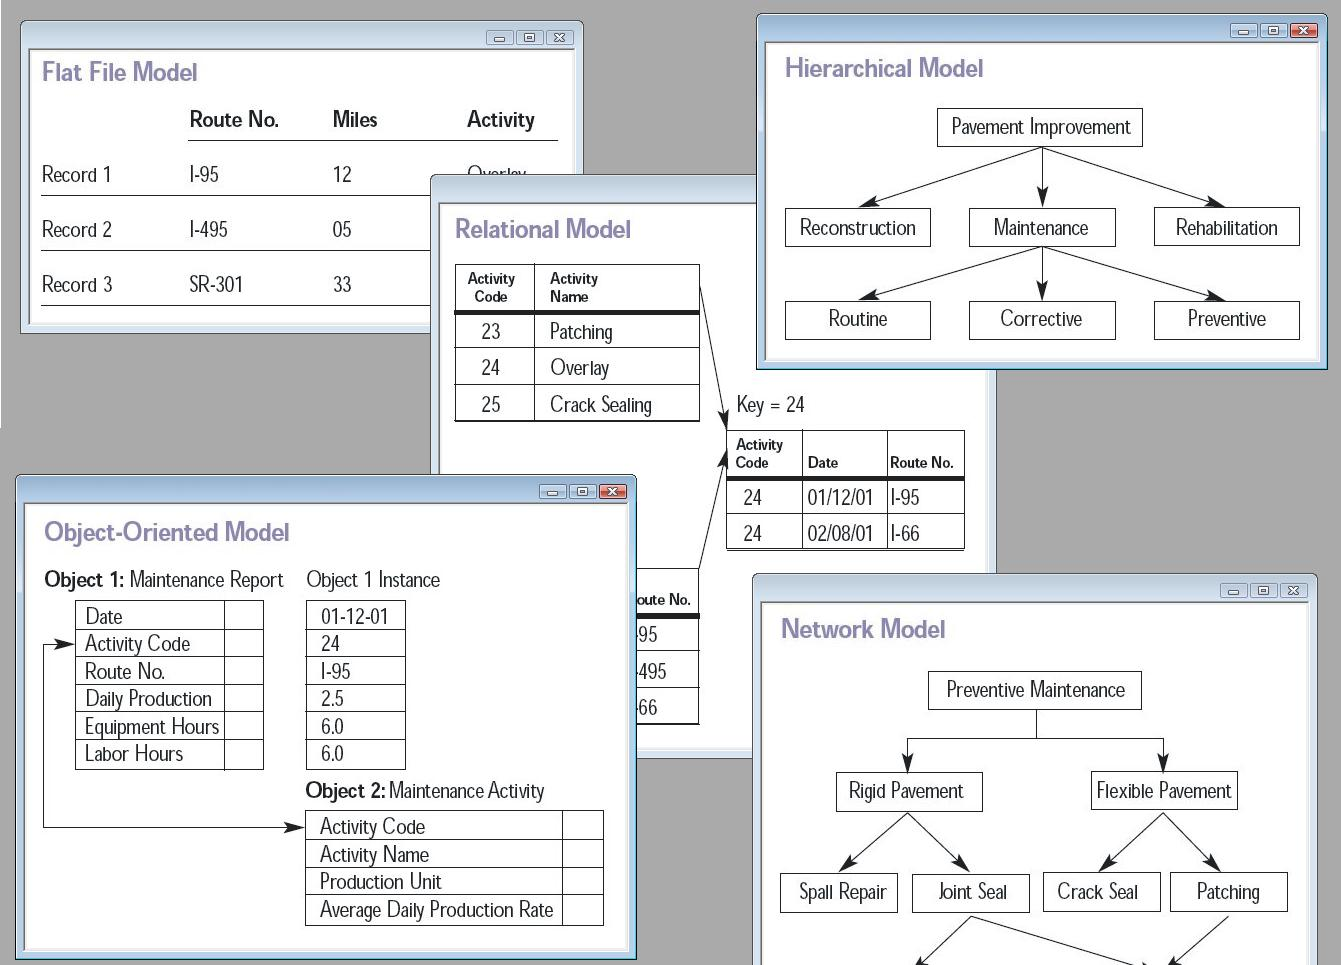
\includegraphics[keepaspectratio]{course-contents/images/database-models.png}}

}

\caption{Wikipedia 2016 Database Models}

\end{figure}%

Wikipedia (2016)

\section{Document databases}\label{document-databases}

Most well known example is mongodb. Document databases mostly store json
documents. They are schema-free organization of data. That is unlike the
relational databases, you do not upfront have to design database schema.

This has advantages and disadvantages.

Examples include

\begin{itemize}
\tightlist
\item
  MongoDB
\item
  Databricks
\item
  Amazon DynamoDB
\item
  Microsoft Azure Cosmos DB
\item
  Couchbase
\item
  Firebase (google)
\item
  Oracle NoSQL
\end{itemize}

\section{Graph Database}\label{graph-database}

\begin{figure}[H]

{\centering \pandocbounded{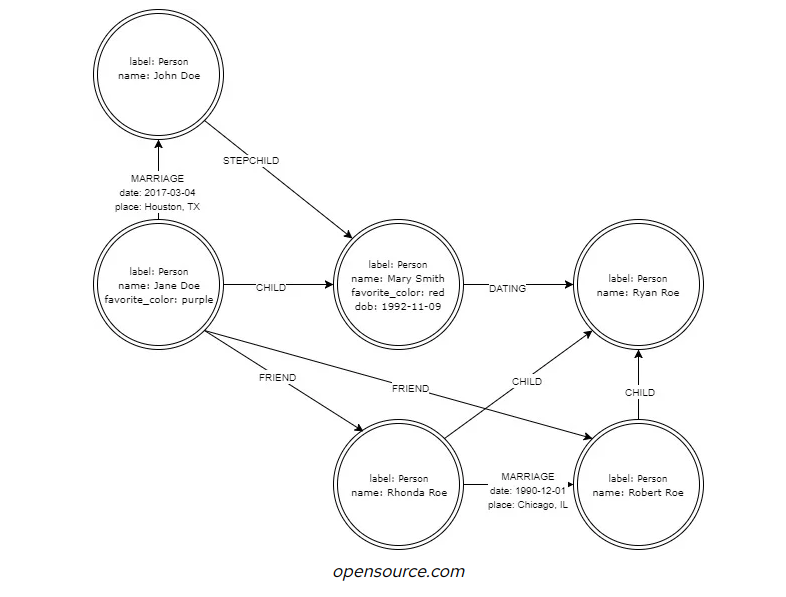
\includegraphics[keepaspectratio]{course-contents/./images/database-models-graph-example-opensource-com.png}}

}

\caption{Wikipedia2016DatabaseModelsFigure}

\end{figure}%

\section{Vector databases}\label{vector-databases}

\includegraphics[width=4.52in,height=8in]{course-contents/database-models-en_files/figure-latex/mermaid-figure-1.png}

\part{Causality}

\chapter{Entity Relationship (ER)
modelling}\label{entity-relationship-er-modelling}

\section{Entity Relationship modeling
Basics}\label{entity-relationship-modeling-basics}

Entity Relationship (ER) modeling or diagramming is introduce by Peter
Chen Chen (1976) in 1976. ER-Models consists of three parts

\begin{itemize}
\tightlist
\item
  Entity
\item
  Relations
\item
  Attributes
\end{itemize}

Entities are basically tables in databases, like Student, Employee,
Customer and Invoices. Relations shows the connections between entities.
For example, a Customer has invoices. Attributes shows the values an
entity have: For example, Customer entity will have name and phone.

Original syntax is called Chen notation. Below is an figure from the
original article Chen (1976).

\begin{figure}[H]

{\centering 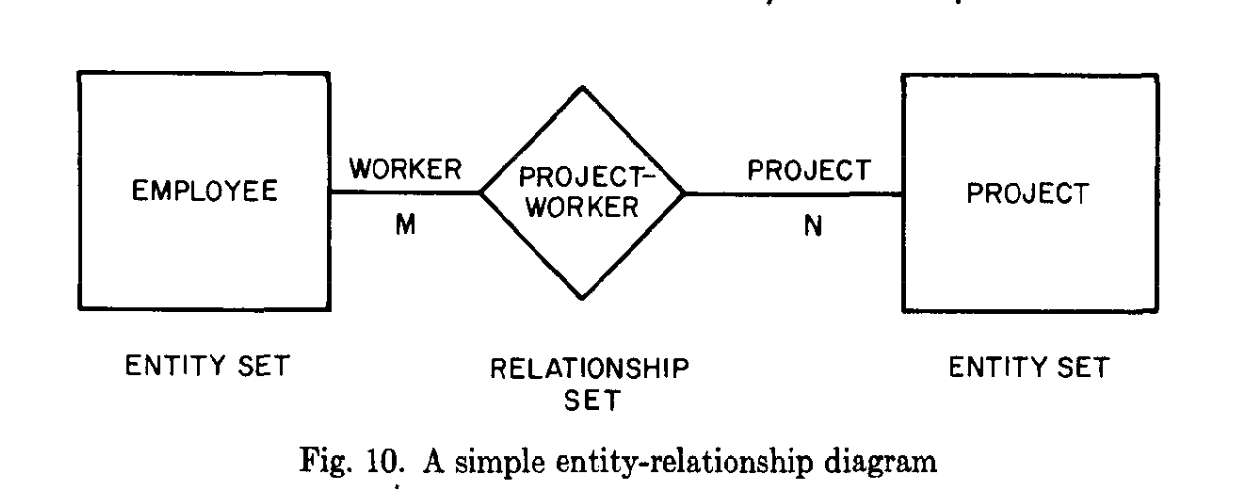
\includegraphics[width=0.8\linewidth,height=\textheight,keepaspectratio]{course-contents/images/Chen-1976-Figure-10-simple-er-diagram.png}

}

\caption{Simple Er Diagram}

\end{figure}%

The diagramming syntax is evolved by then but the basics stayed same.

\section{How it works}\label{how-it-works}

ER-modelling work two ways, as below figure shows. First way, we could
create diagrams then database tables. Second way, we could reverse
engineer our diagrams from our database tables.

\includegraphics[width=4.32in,height=2.06in]{course-contents/er-model-en_files/figure-latex/mermaid-figure-1.png}

\section{ER Modelling tools}\label{er-modelling-tools}

For first way, there are a lot of tools exits. Examples:

\begin{itemize}
\tightlist
\item
  \href{https://sparxsystems.com/products/ea/}{Enterprise Architect}
\item
  \href{https://blog.toadworld.com/what-an-er-diagram-is-and-tools-that-help-build-and-alter-them}{Toad}
\item
  \href{https://www.lucidchart.com/pages/er-diagrams}{LucidChart ER
  Diagrams}
\end{itemize}

See following video for how one tool works.
\href{https://www.youtube.com/watch?v=RBZtPhZkUZM}{LucidChart Tutorial:
How to Create an ERD}

\section{ER model reverse engineering
tools}\label{er-model-reverse-engineering-tools}

Second way of working, reverse engineering existing database is more
common. We reverse engineer an already existing database and get ER
Diagram of it. For example, DBeaver has ER Diagrams.

\begin{figure}[H]

{\centering \pandocbounded{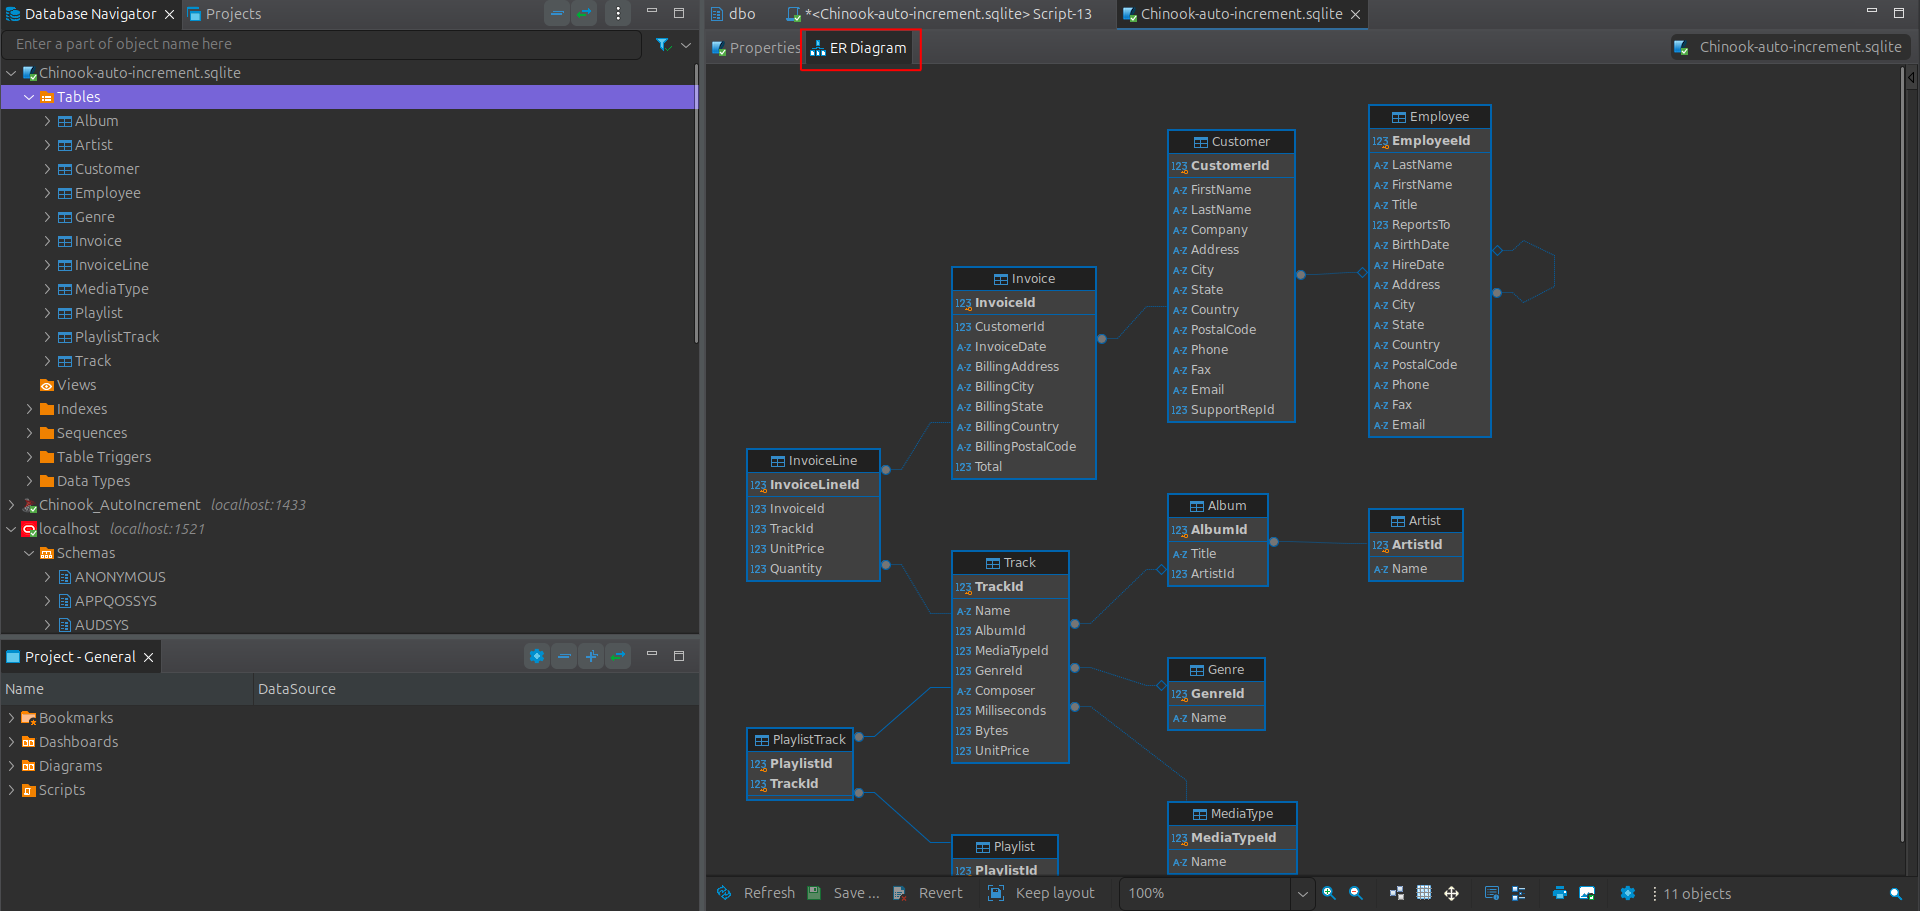
\includegraphics[keepaspectratio]{course-contents/images/dbeaver-er-diagram.png}}

}

\caption{DBeaver ER Diagram}

\end{figure}%

\begin{enumerate}
\def\labelenumi{\arabic{enumi}.}
\tightlist
\item
  Open a connection
\item
  select tables
\item
  in the opened window, select ER Diagram tab
\end{enumerate}

Reading ER diagrams is useful skill to have since it allows you to more
easily understand existing database structure.

\href{https://docs.oracle.com/en/database/oracle/oracle-database/18/comsc/schema-diagrams.html\#GUID-01BFEF14-C6BD-42CD-8558-DDD214DB3AE0}{See
oracle sample HR and OE example in their documentation}

Oracle SQL Developer has its own reverse engineering tools for oracle
database. TODO add links.

Another tool for this purpose is Schema Spy.

\chapter{Mermaid ER Diagrams}\label{mermaid-er-diagrams}

We use
\href{https://mermaid.js.org/syntax/entityRelationshipDiagram.html}{mermaid
Entity Relationship Diagram} for diagramming since markdown syntax of
mermaid is more easily understood and markdown as plain text is version
controllable with source control tools like git. Also mermaid diagrams
are automatically rendered by web versions of source control tools such
as github, gitlab and azure devops.

\section{Entity}\label{entity}

Entities are most basic part in the diagrams. They correspond to
database tables normally. We can also give their attributes or columns
in the diagram too. See below example.

\begin{Shaded}
\begin{Highlighting}[]
\NormalTok{erDiagram}
\NormalTok{    Student \{}
\NormalTok{        int student\_id PK}
\NormalTok{        string name}
\NormalTok{    \}}
\end{Highlighting}
\end{Shaded}

\includegraphics[width=1.62in,height=1.13in]{course-contents/er-model-mermaid-diagrams-en_files/figure-latex/mermaid-figure-1.png}

\section{Entity Relationships}\label{entity-relationships}

Entities should have relationships. That is how they interact with other
entities. The syntax for it is below:

\begin{verbatim}
<first-entity> [<relationship> <second-entity> : <relationship-label>]
\end{verbatim}

Relationship label should show how it works in the requirements or
domain. Please try to choose it accordingly.

An example a student enrolls in many courses. We could write it like
below.

\begin{Shaded}
\begin{Highlighting}[]
\NormalTok{erDiagram}
\NormalTok{    Student ||{-}{-}o\{ Course : enrolls}
\end{Highlighting}
\end{Shaded}

\includegraphics[width=1.46in,height=3.02in]{course-contents/er-model-mermaid-diagrams-en_files/figure-latex/mermaid-figure-3.png}

In this syntax, following table shows how we can model cardinality of
the entities. That is 0,1 or many information between the entities.

\begin{longtable}[]{@{}lll@{}}
\toprule\noalign{}
Value (left) & Value (right) & Meaning \\
\midrule\noalign{}
\endhead
\bottomrule\noalign{}
\endlastfoot
\textbar o & o\textbar{} & Zero or one \\
\textbar\textbar{} & \textbar\textbar{} & Exactly one \\
\}o & o\{ & Zero or more (no upper limit) \\
\}\textbar{} & \textbar\{ & One or more (no upper limit) \\
\end{longtable}

We can read this information following way then

\begin{itemize}
\tightlist
\item
  Student has zero to one advisor
\item
  Student has exactly one advisor
\item
  Student enrolls in 0-to-many courses
\item
  Student enrolls in 1-to-many courses
\end{itemize}

\section{Full example 1}\label{full-example-1}

\begin{Shaded}
\begin{Highlighting}[]
\NormalTok{erDiagram}
\NormalTok{    STUDENT ||{-}{-}o\{ COURSE : enrolls}
\NormalTok{    COURSE ||{-}{-}|\{ LESSON : contains}
\NormalTok{    TEACHER ||{-}{-}o\{ COURSE : teaches}
\NormalTok{    TEACHER ||{-}{-}o\{ LESSON : conducts}
\NormalTok{    STUDENT ||{-}{-}o\{ LESSON : attends}


\NormalTok{    STUDENT \{}
\NormalTok{        int id PK}
\NormalTok{        string name}
\NormalTok{        date created\_at}
\NormalTok{        date updated\_at}
\NormalTok{    \}}
\NormalTok{    COURSE \{}
\NormalTok{        int id PK}
\NormalTok{        string title}
\NormalTok{        string description}
\NormalTok{        date created\_at}
\NormalTok{        date updated\_at}
\NormalTok{    \}}
\NormalTok{    LESSON \{}
\NormalTok{        int id PK}
\NormalTok{        int course\_id FK}
\NormalTok{        string title}
\NormalTok{        date scheduled\_date}
\NormalTok{        date created\_at}
\NormalTok{        date updated\_at}
\NormalTok{    \}}
\NormalTok{    TEACHER \{}
\NormalTok{        int id PK}
\NormalTok{        string name}
\NormalTok{        string email}
\NormalTok{        date created\_at}
\NormalTok{        date updated\_at}
\NormalTok{    \}}
\end{Highlighting}
\end{Shaded}

\includegraphics[width=5.12in,height=6.92in]{course-contents/er-model-mermaid-diagrams-en_files/figure-latex/mermaid-figure-2.png}

https://mermaid.live/

\section{Use LLMs to generate ER
diagrams}\label{use-llms-to-generate-er-diagrams}

We can use LLMs like ChatGPT, Gemini or Perplexity to create our draft
diagrams since mermaid is normal markdown code.

Below AI prompt creates a draft mermaid diagram to start from.

\begin{quote}
Please create me a simple mermaid entity relationship diagram which
shows students, courses, lessons and teachers. All of the entities
should have common columns in it.
\end{quote}

Try it in AI tools to see the result.

\part{SQL Intro}

\chapter{Why learn SQL Language?}\label{why-learn-sql-language}

\section*{Reason 1: SQL is popular and widely
used}\label{reason-1-sql-is-popular-and-widely-used}
\addcontentsline{toc}{section}{Reason 1: SQL is popular and widely used}

\markright{Reason 1: SQL is popular and widely used}

SQL is the \href{https://www.tiobe.com/tiobe-index/sql/}{number 8 in the
tiobe index}. Note that, SQL is new in this list since it was not
considered programming language before 2018. But as
\href{https://www.tiobe.com/tiobe-index/}{same web page} says

\begin{quote}
The programming language SQL was added to the TIOBE index in 2018 after
somebody pointed out that SQL is Turing Complete. So although this
language is very old, it has only a short history in the index.
\end{quote}

\href{https://github.com/nuno-faria/tetris-sql}{SQL Tetris in Postgresql
for turing complete example}

\section*{Reason 2: SQL is widely asked in job
advertisements}\label{reason-2-sql-is-widely-asked-in-job-advertisements}
\addcontentsline{toc}{section}{Reason 2: SQL is widely asked in job
advertisements}

\markright{Reason 2: SQL is widely asked in job advertisements}

\begin{itemize}
\tightlist
\item
  \href{https://www.stepstone.de/work/sql?searchOrigin=Homepage_top-search}{stepstone.de
  Germany}
\item
  \href{https://www.indeed.com/jobs?q=sql&fromage=last&sc=0kf\%3Aattr\%28FGY89\%29\%3B&vjk=24f6984f2ffca44a}{indeed.com
  USA}
\item
  \href{https://www.kariyer.net/is-ilanlari?kw=sql}{kariyer.net Türkiye}
\end{itemize}

\section*{Reason 3: SQL is used in places other than
databases}\label{reason-3-sql-is-used-in-places-other-than-databases}
\addcontentsline{toc}{section}{Reason 3: SQL is used in places other
than databases}

\markright{Reason 3: SQL is used in places other than databases}

SQL widely used in data science with databases and in memory data
frames. Data frames are in memory tables. Both python and R has
different data frame implementations. You could use SQL to create data
frames from databases and query data frames themselves. See below:

\begin{itemize}
\item
  \href{https://stackoverflow.com/questions/45865608/executing-an-sql-query-on-a-pandas-dataset}{Query
  python pandas data frame}
\item
  \href{https://www.rdocumentation.org/packages/sqldf/versions/0.4-11}{Query
  R Data frame}
\end{itemize}

SQL is also used for other use cases like querying logs.

\begin{itemize}
\tightlist
\item
  \href{https://techcommunity.microsoft.com/t5/exchange-team-blog/introducing-log-parser-studio/ba-p/601131}{Query
  logs using SQL via log parser}
\end{itemize}

Also, querying csv and excel files using SQL is possible.

\begin{itemize}
\item
  \href{https://superuser.com/questions/7169/querying-a-csv-file}{Query
  csv files using SQL}
\item
  \href{https://stackoverflow.com/questions/18798522/how-to-run-a-sql-query-on-an-excel-table}{Query
  excel files using SQL}
\item
  \href{https://osquery.readthedocs.io/en/stable/}{osquery: Query system
  data using SQL}
\end{itemize}

\begin{quote}
osquery exposes an operating system as a high-performance relational
database. This allows you to write SQL queries to explore operating
system data. With osquery, SQL tables represent abstract concepts such
as running processes, loaded kernel modules, open network connections,
browser plugins, hardware events or file hashes.
\end{quote}

\section*{Reason 4: SQL is better compared to newer query
languages}\label{reason-4-sql-is-better-compared-to-newer-query-languages}
\addcontentsline{toc}{section}{Reason 4: SQL is better compared to newer
query languages}

\markright{Reason 4: SQL is better compared to newer query languages}

See below:

\begin{itemize}
\tightlist
\item
  \href{https://antonz.org/fancy-ql/}{I don't need your query language}
\end{itemize}

\chapter{SQL history}\label{sql-history}

\begin{itemize}
\item
  SQL is developed at IBM in the 1970s by Donald D. Chamberlin and
  Raymond F. Boyce.
\item
  SQL is based on the article of Edgar F. Codd ``A Relational Model of
  Data for Large Shared Data Banks'' Codd (1970)
\item
  Entity-relationship model introduced by Chen.
\item
  First commercial version was released by Oracle in 1979.
\item
  Although it is defined as declarative, it also has procedural
  elements.
\item
\end{itemize}

\part{Database Concepts}

\chapter{Database Concepts ACID}\label{database-concepts-acid}

ACID is an acronym for \textbf{A}tomicity, \textbf{C}onsistency,
\textbf{I}solation, \textbf{D}urability. ACID is fundamental concept for
relational database systems for reliable transactions. Conformance ACID
concepts is what makes a relational database a must requirement for some
software systems like banking.

\textbf{Atomicity}

Atomicity guarantees that a transaction is a single unit. All commands
within this transaction are either all succesful or they are all rolled
backed. Rolling back a transaction is like it is never executed at all.
For example, consider money transfer in a bank. Executing following
code.

\begin{Shaded}
\begin{Highlighting}[]
\ControlFlowTok{BEGIN} \KeywordTok{TRANSACTION}    
    \KeywordTok{UPDATE} \KeywordTok{Account}
    \KeywordTok{SET}\NormalTok{ Money }\OperatorTok{=}\NormalTok{ Money }\OperatorTok{{-}}\DecValTok{100}
    \KeywordTok{WHERE}\NormalTok{ Owner }\OperatorTok{=}\NormalTok{ A;}
    \KeywordTok{UPDATE} \KeywordTok{Account}
    \KeywordTok{SET}\NormalTok{ Money }\OperatorTok{=}\NormalTok{ Money }\OperatorTok{+}\DecValTok{100}
    \KeywordTok{WHERE}\NormalTok{ Owner }\OperatorTok{=}\NormalTok{ B;}

\KeywordTok{COMMIT} \KeywordTok{TRANSACTION}    
\end{Highlighting}
\end{Shaded}

Atomicity guarantees that both of these updates are successful or both
of them rolled back. This roll back could occur due to failure of one of
the commands. For example, we could have a constraint or trigger which
prevents negative values for money in Account table.

Atomicity prevents inconsistencies like not decreasing money from
Account A but increasing money of Account B.

\textbf{Consistency}

Consistency guarantees that a transaction preserves valid states. That
is after the transaction database is in a valid state. Consistency
enforces database constraints like primary keys, foreign keys and other
constraints. For example, we are adding a invoice and invoice lines.
Invoice lines are dependent upon (have foreign keys) invoice table. If
adding a invoice is not successful, we could not add invoice lines also.

\textbf{Isolation}

Isolation guarantees that multiple transactions occur concurrently
without seeing each other. For example, one transaction update a row in
Customer table, second transaction will not see this update row.

Isolation prevents Read Phenomenas of dirty reads,non-repeatable reads
and phantom reads. For example, isolation ensures that two users could
not change same row at the same time.

\textbf{Durability}

Durability guarantees that committed transaction will stay in disk even
in the system crashes, power failures or other problems. For example,
durability ensures that when a bank transfer is successful, all account
changes are permanently preserved in the database system.

The ACID properties collectively ensures that database transactions
works reliably. Implementing ACID properties introduce performance
penalties. That is why most NoSQL databases are faster since they
implement ACID properties more weakly compared to traditional relational
database systems. If your system needs ACID guarantees, relational
databases are always safer choice.

\chapter{isolation}\label{isolation}

Isolation is the I of ACID acronym.

As mentioned before, Isolation guarantees that multiple transactions
occur concurrently without seeing each other. For example, one
transaction update a row in Customer table, second transaction will not
see this update row.

Isolation prevents Read Phenomenas of dirty reads,non-repeatable reads
and phantom reads. For example, isolation ensures that two users could
not change same row at the same time.

\begin{longtable}[]{@{}
  >{\raggedright\arraybackslash}p{(\linewidth - 6\tabcolsep) * \real{0.4405}}
  >{\raggedright\arraybackslash}p{(\linewidth - 6\tabcolsep) * \real{0.1429}}
  >{\raggedright\arraybackslash}p{(\linewidth - 6\tabcolsep) * \real{0.2500}}
  >{\raggedright\arraybackslash}p{(\linewidth - 6\tabcolsep) * \real{0.1667}}@{}}
\toprule\noalign{}
\begin{minipage}[b]{\linewidth}\raggedright
Isolation level vs Read phenomenon
\end{minipage} & \begin{minipage}[b]{\linewidth}\raggedright
Dirty read
\end{minipage} & \begin{minipage}[b]{\linewidth}\raggedright
Non-repeatable read
\end{minipage} & \begin{minipage}[b]{\linewidth}\raggedright
Phantom read
\end{minipage} \\
\midrule\noalign{}
\endhead
\bottomrule\noalign{}
\endlastfoot
Serializable & no & no & no \\
Repeatable read & no & no & yes \\
Read committed & no & yes & yes \\
Read uncommitted & yes & yes & yes \\
\end{longtable}

Most relational databases support serializable isolation by default
since it prevents read phenomenas.

\begin{itemize}
\tightlist
\item
  Sqlite transactions are serializable
\item
  Changes made in one database connection is not visible to all other
  database connections
\item
  A query sees the state of the database prior to start of the query.
  That is all transactions completed before the query runs.
\end{itemize}

In addition to serializable isolation, some databases support
\href{https://en.wikipedia.org/wiki/Snapshot_isolation}{Snapshot
isolation}. Snapshot isolation guarantees that reads in a transaction
will see a consistent snapshot of the database. Different from
serializable, transactions in the snapshot isolation will only commit if
there is no conflicting update done after that snapshot. Actually, this
means that if same rows are changed by two different transactions,
second transaction will be rolled back. Snapshot isolation has better
performance than serializable isolation. Snapshot isolation is supported
by Oracle, MySQL, PostgreSQL, Microsoft SQL Server.

\begin{tcolorbox}[enhanced jigsaw, titlerule=0mm, colback=white, colbacktitle=quarto-callout-caution-color!10!white, toprule=.15mm, coltitle=black, opacitybacktitle=0.6, left=2mm, leftrule=.75mm, arc=.35mm, title=\textcolor{quarto-callout-caution-color}{\faFire}\hspace{0.5em}{Caution}, breakable, colframe=quarto-callout-caution-color-frame, bottomtitle=1mm, rightrule=.15mm, toptitle=1mm, opacityback=0, bottomrule=.15mm]

Snapshot isolation is called serializable by Oracle and PostgreSQL
(prior to 9.1)

\end{tcolorbox}

\begin{itemize}
\tightlist
\item
  \href{https://en.wikipedia.org/wiki/Isolation_\%28database_systems\%29}{Isolation
  in wikipedia}
\item
  \href{https://sqlite.org/isolation.html}{Isolation in sqlite}
\item
  \href{https://learn.microsoft.com/en-us/sql/t-sql/language-elements/transaction-isolation-levels?view=sql-server-ver16}{Isolation
  in SQL Server}
\item
  \href{https://learn.microsoft.com/en-us/sql/t-sql/statements/set-transaction-isolation-level-transact-sql?view=sql-server-ver16}{SET
  TRANSACTION ISOLATION LEVEL (Transact-SQL)}
\item
  \href{https://docs.oracle.com/en/database/oracle/oracle-database/19/cncpt/data-concurrency-and-consistency.html\#GUID-4BD4DFD6-DAEA-41B2-BB56-7135568F0548}{Isolation
  in Oracle}
\item
  \href{https://en.wikipedia.org/wiki/Snapshot_isolation}{snapshot
  isolation in wikipedia}
\end{itemize}

\part{Database Design Advanced}

\chapter{Database design}\label{database-design}

We will first work with practical examples. Then lastly we will cover
theory of database normalization.

\chapter{Primary Key}\label{primary-key}

In relational databases, primary keys identify the records in a table as
unique. The benefit of finding a record as unique is that querying and
updating this record is much faster with this key. Similarly,
relationships between tables are maintained by foreign keys that are
linked to primary keys.

For example, suppose we have PERSON and PERSON\_TRAINING tables. Which
trainings a person has received is tracked using the Person primary key
in the PERSON\_TRAINING table. Therefore, primary key selection is very
important in database design.

There are 2 different ideas in primary key selection: Natural Key and
Synthetic Key.

Before explaining the differences, pros and cons between the two, let me
state that I am in favor of synthetic keys.

\section{Natural Key}\label{natural-key}

Natural Key proponents recommend choosing a primary key based on
information that already exists in the domain when designing a database.
Since users are already familiar with this information, natural keys
will be much easier to use and adopt. These keys are also easier to use
by people who are not familiar with database logic.

In table
Table~\ref{tbl-table-primary-key-natural-key-example-city-table},
license plateCode is selected as the primary key.

\begin{longtable}[]{@{}cc@{}}
\caption{Natural Key Example 1 - City
Table}\label{tbl-table-primary-key-natural-key-example-city-table}\tabularnewline
\toprule\noalign{}
CITY & \\
\midrule\noalign{}
\endfirsthead
\toprule\noalign{}
CITY & \\
\midrule\noalign{}
\endhead
\bottomrule\noalign{}
\endlastfoot
PlateCode & PK \\
CityName & \\
\end{longtable}

The advantage of Natural Keys is that they are already known as I
mentioned before. As a disadvantage, since these keys have meaning in
the domain, our database schema has become domain dependent. Keys need
to be changed in requirement changes. For example, let's assume that
TcIdentityNo is selected as the primary key in Table
Table~\ref{tbl-table-primary-key-natural-key-example-person}. If this
key is entered incorrectly in the first entry, it will be necessary to
change this information entered as Foreign Key in all tables connected
to this key, for example (PERSON\_TRAINING, PERSON\_EXPERIENCE).

\begin{longtable}[]{@{}cc@{}}
\caption{Natural Key Example 2 - Person
Table}\label{tbl-table-primary-key-natural-key-example-person}\tabularnewline
\toprule\noalign{}
PERSON & \\
\midrule\noalign{}
\endfirsthead
\toprule\noalign{}
PERSON & \\
\midrule\noalign{}
\endhead
\bottomrule\noalign{}
\endlastfoot
TcIdentityNo & PK \\
FirstName & \\
LastName & \\
\end{longtable}

In table
Table~\ref{tbl-table-primary-key-natural-key-example-address-table}, a
somewhat extreme example is the Address table. It is difficult to find a
suitable natural key in the address table, so all the information
entered had to be made as a composite key.

\begin{longtable}[]{@{}cc@{}}
\caption{Natural Key Example 3 - Address
Table}\label{tbl-table-primary-key-natural-key-example-address-table}\tabularnewline
\toprule\noalign{}
ADDRESS & \\
\midrule\noalign{}
\endfirsthead
\toprule\noalign{}
ADDRESS & \\
\midrule\noalign{}
\endhead
\bottomrule\noalign{}
\endlastfoot
AddressLine1 & PK \\
AddressLine1 & PK \\
ApartmentName & PK \\
ApartmentNo & PK \\
PostalCode & PK \\
County & PK \\
CityNo & PK \\
CountryNo & PK \\
\end{longtable}

\section{Surrogate Key}\label{surrogate-key}

Instead of selecting a Natural Key, automatically generated keys can be
used as primary keys. The advantage is that if the natural key changes,
the records in the database are not affected by this situation. Another
advantage is that even in case of lack of information in the initial
data entries, data can be recorded with the existing information. Others
are the convenience in back-end programming and queries.

In the example given earlier with PERSON and TcIdentityNo in the natural
key, if TcIdentityNo changes will only affect the PERSON table. In this
case, de-coupling will be provided between the domain and the
application.

But the most effective argument for the synthetic key is the convenience
it brings to programmers. It makes it easier to write code with the
appropriate strategy.

The disadvantage of synthetic keys is that they are often less
understandable. This is especially true for universally unique
identifiers (UUID/GUID).

In table
Table~\ref{tbl-table-primary-key-synthetic-key-sample-person-table},
KisiKey is selected as synthetic key. In this table, duplicate entries
of TcKimlikNo can be prevented by adding a unique index on TcKimlikNo

\begin{longtable}[]{@{}cc@{}}
\caption{Synthetic Key Example - Person
Table}\label{tbl-table-primary-key-synthetic-key-sample-person-table}\tabularnewline
\toprule\noalign{}
PERSON & \\
\midrule\noalign{}
\endfirsthead
\toprule\noalign{}
PERSON & \\
\midrule\noalign{}
\endhead
\bottomrule\noalign{}
\endlastfoot
PersonKey & PK \\
TcIdentityNo & \\
FirstName & \\
LastName & \\
\end{longtable}

One of the important points to note about synthetic keys is that they
should not be used to add business meaning. For example, the company
numbers given to companies by chambers of commerce are usually a
synthetic key generated by databases. But in the below example, they are
given a business meaning.

An example of this can be seen in the figure
Figure~\ref{fig-synthetic-key-used-like-natural-key}. This example is
taken from an old version of chamber of commerce software. How true or
false this situation is is a matter of debate.

\begin{figure}

\centering{

\pandocbounded{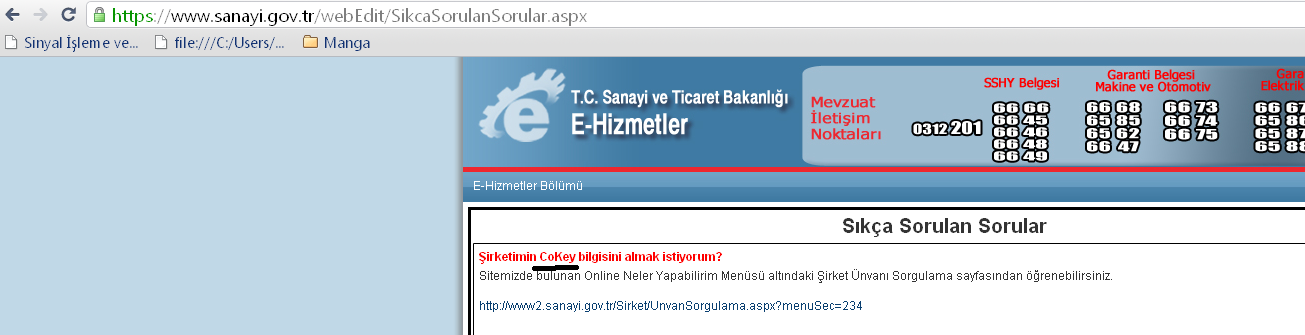
\includegraphics[keepaspectratio]{course-contents/./images/sentetik-anahtarin-dogal-anahtar-gibi-kullanilmasi.png}}

}

\caption{\label{fig-synthetic-key-used-like-natural-key}}

\end{figure}%

The Synthetic Key vs.~Natural Key debate has turned into a religious
debate in some places. Remember that there is never one right way to
design a database. It is your application. Choose the most appropriate
strategy according to your requirements.

\section{Auto number (identity)}\label{auto-number-identity}

The synthetic key can be generated on the database side or on the
application side that accesses the database. The most preferred form of
synthetic key on the database side is automatic number generation. This
Auto Number strategy is supported by many databases:

\begin{itemize}
\tightlist
\item
  Sqlite
\item
  SQL Server
\item
  Oracle 12c+
\item
  MySQL
\item
  IBM DB2
\end{itemize}

Auto Number columns are bound to the database table and each time an
Insert clause is executed, the next automatically generate the value.

\section{Sequences}\label{sequences}

If auto number generated by database is used in more than one table,
sequences will be more useful. Sequences are database objects from which
users may generate unique integers.

\begin{itemize}
\tightlist
\item
  \href{https://docs.oracle.com/en/database/oracle/oracle-database/21/sqlrf/CREATE-SEQUENCE.html}{oracle
  sequences}
\item
  \href{https://learn.microsoft.com/en-us/sql/t-sql/statements/create-sequence-transact-sql?view=sql-server-ver16}{Sql
  server sequences}
\end{itemize}

\part{SQL Tuning}

\chapter{SQL indexes introduction}\label{sql-indexes-introduction}

\section{Indexes are like book
indexes}\label{indexes-are-like-book-indexes}

TODO

\section{B+ Tree}\label{b-tree}

\begin{itemize}
\tightlist
\item
  \href{https://www.cs.usfca.edu/~galles/visualization/BPlusTree.html}{Very
  good B+ Tree visualization}
\end{itemize}

\section{Sqlite}\label{sqlite}

https://www.sqlite.org/lang\_createindex.html

\section{Other tutorials or lessons
(Optional)}\label{other-tutorials-or-lessons-optional}

Below tutorials are extra information for interested students

\begin{itemize}
\tightlist
\item
  \href{https://www.youtube.com/watch?v=scUtG_6M_lU}{08 - Tree Indexes:
  B+Trees (CMU Intro to Database Systems)}
\end{itemize}

\bookmarksetup{startatroot}

\chapter{Suggested Readings}\label{suggested-readings}

Databases are a very necessary skill to have for developers. See
following readings about this topic:

\begin{itemize}
\item
  \href{https://www.simplethread.com/relational-databases-arent-dinosaurs-theyre-sharks/}{Relational
  Databases Aren't Dinosaurs, They're Sharks}
\item
  \href{https://spectrum.ieee.org/the-rise-of-sql}{The Rise of SQL: It's
  become the second programming language everyone needs to know}
\item
  \href{https://www.tiobe.com/tiobe-index/sql/}{Tiobe Index SQL}
\item
  \href{https://antonz.org/fancy-ql/}{I don't need your query language}
\item
  \href{../reference-documents/1983_A\%20simple\%20guide\%20to\%20five\%20normal\%20forms\%20in\%20relational\%20database\%20theory_Annotated.pdf}{A
  simple guide to five normal forms in relational database theory}
\end{itemize}

Hopefully, at the end of this course, you will know about everything in
the following article:

\begin{itemize}
\tightlist
\item
  \href{https://architecturenotes.co/things-you-should-know-about-databases/}{Things
  you should know about databases}
\end{itemize}

\bookmarksetup{startatroot}

\chapter{Suggested Books}\label{suggested-books}

Following books are recommended but they are not necessary to pass the
course. I am recommending them if you want to be a better developer or
database administrator.

\begin{itemize}
\item
  \href{https://www.amazon.com/Database-Design-Mere-Mortals-Anniversary/dp/0136788041}{Database
  Design for Mere Mortals: 25th Anniversary Edition}
\item
  \href{https://use-the-index-luke.com/}{SQL Performance Explained}
\end{itemize}

\bookmarksetup{startatroot}

\chapter*{References}\label{references-1}
\addcontentsline{toc}{chapter}{References}

\markboth{References}{References}

\phantomsection\label{refs}
\begin{CSLReferences}{1}{0}
\bibitem[\citeproctext]{ref-Chen1976entity}
Chen, Peter Pin-Shan. 1976. {``The Entity-Relationship Model---Toward a
Unified View of Data.''} \emph{ACM Transactions on Database Systems} 1
(1): 9--36. \url{https://doi.org/10.1145/320434.320440}.

\bibitem[\citeproctext]{ref-Codd1970relational}
Codd, E. F. 1970. {``A Relational Model of Data for Large Shared Data
Banks.''} \emph{Communications of the ACM} 13 (6): 377--87.
\url{https://doi.org/10.1145/362384.362685}.

\bibitem[\citeproctext]{ref-knuth84}
Knuth, Donald E. 1984. {``Literate Programming.''} \emph{Comput. J.} 27
(2): 97--111. \url{https://doi.org/10.1093/comjnl/27.2.97}.

\bibitem[\citeproctext]{ref-Wikipedia2016DatabaseModelsFigure}
Wikipedia. 2016. {``DatabaseModelsFigure --- Wikipedia{,} the Free
Encyclopedia.''}

\end{CSLReferences}




\end{document}
